\documentclass{article}
\PassOptionsToPackage{table}{xcolor}
\usepackage{amssymb}
\usepackage{geometry}
\usepackage{tikz}
\usepackage[most]{tcolorbox}
\usepackage{mathabx}
\usepackage{booktabs}
\usepackage{tabularx}
\usepackage{nicefrac}
\usepackage{pdflscape}
\usepackage{fontawesome}

\usetikzlibrary{tikzmark}

\geometry{a4paper, total={170mm, 257mm}, left=20mm}
\linespread{1.9}

\tcbset{on line, box align=base,
    sharp corners=northwest,sharp corners=southeast,
    boxsep=4pt, left=0pt,right=0pt,top=0pt,bottom=0pt,
    grow to left by=5pt,
    colframe=white
}
\newcommand{\splitbox}[3]{
    \tcbox[enhanced, interior code={%
        \path[fill=#1,rounded corners=5px] (interior.north west) |- (interior.south east);
        \path[fill=#2,rounded corners=5px] (interior.south east) |- (interior.north west);
    }]{#3}
}

\colorlet{instr-arg}{red!30!green!20}
\colorlet{instr-jsp}{blue!90!green!20}
\colorlet{instr-mem}{red!90!blue!20}
\colorlet{instr-u32}{teal!20}
\colorlet{row1}{white}
\colorlet{row2}{gray!8}

\begin{document}
\pagestyle{empty}
\hfill
\begin{tikzpicture}[overlay]
    \node[anchor=north east, inner sep=0] at (1,1.5) {
        \includegraphics[keepaspectratio,width=0.4\textwidth]{src/img/triton-logo.pdf}
    };
    \node[anchor=north east, inner sep=0] at (1,0) {\texttt{\LARGE v0.18}};
\end{tikzpicture}

{
\renewcommand{\arraystretch}{0.84}
\begin{tabular}{rllll}
    \texttt{  2} & $\ominus$     & \texttt{pop}                                       & \texttt{\_ st$_0$}                                                        & \texttt{\_}                                                                \\
    \texttt{  1} & $\oplus$      & \tcbox[colback=instr-arg]{\texttt{push + a}}       & \texttt{\_}                                                               & \texttt{\_ a}                                                              \\
    \texttt{  8} & $\oplus$      & \texttt{divine}                                    & \texttt{\_}                                                               & \texttt{\_ a}                                                              \\
    \texttt{  9} & $\oplus$      & \tcbox[colback=instr-arg]{\texttt{dup + i}}        & \texttt{\_ st$_{15}$ $\dots$ st$_0$}                                      & \texttt{\_ st$_{15}$ $\dots$ st$_0$ st$_i$}                                \\
    \texttt{ 17} & $\ovoid^{16}$ & \tcbox[colback=instr-arg]{\texttt{swap + i}}       & \texttt{\_ $\dots$ st$_i$ $\dots$ st$_0$}                                 & \texttt{\_ $\dots$ st$_0$ $\dots$ st$_i$}                                  \\
    \texttt{ 16} & $\ovoid$      & \texttt{nop}                                       & \texttt{\_}                                                               & \texttt{\_}                                                                \\
    \texttt{ 10} & $\ominus$     & \tcbox[colback=instr-jsp]{\texttt{skiz}}           & \texttt{\_ st$_0$}                                                        & \texttt{\_}                                                                \\
    \texttt{ 25} & $\ovoid$      & \splitbox{instr-jsp}{instr-arg}{\texttt{call + d}} & \texttt{\_}                                                               & \texttt{\_}                                                                \\
    \texttt{ 24} & $\ovoid$      & \tcbox[colback=instr-jsp]{\texttt{return}}         & \texttt{\_}                                                               & \texttt{\_}                                                                \\
    \texttt{ 32} & $\ovoid$      & \tcbox[colback=instr-jsp]{\texttt{recurse}}        & \texttt{\_}                                                               & \texttt{\_}                                                                \\
    \texttt{ 18} & $\ominus$     & \texttt{assert}                                    & \texttt{\_ st$_0$}                                                        & \texttt{\_}                                                                \\
    \texttt{  0} & $\ovoid$      & \texttt{halt}                                      & \texttt{\_}                                                               & \texttt{\_}                                                                \\
    \texttt{ 40} & $\ominus$     & \tcbox[colback=instr-mem]{\texttt{read\_mem}}      & \texttt{\_ addr}                                                          & \texttt{\_ addr a}                                                         \\
    \texttt{ 26} & $\oplus$      & \tcbox[colback=instr-mem]{\texttt{write\_mem}}     & \texttt{\_ addr a}                                                        & \texttt{\_ addr}                                                           \\
    \texttt{ 48} & $\ovoid^{10}$ & \texttt{hash}                                      & \texttt{\_ st$_9$ $\!\!\dots\!\!$ st$_0$}                                 & \texttt{\_ d$_4$ $\!\!\dots\!\!$ d$_0$ 0 $\!\!\dots\!\!$ 0}                \\
    \texttt{ 56} & $\ovoid^{11}$ & \texttt{divine\_sibling}                           & \texttt{\_ idx st$_9$ $\!\!\dots\!\!$ st$_5$ d$_4$ $\!\!\dots\!\!$ d$_0$} & \texttt{\_ idx>>1 r$_4$ $\!\!\dots\!\!$ r$_0$ l$_4$ $\!\!\dots\!\!$ l$_0$} \\
    \texttt{ 64} & $\ovoid$      & \texttt{assert\_vector}                            & \texttt{\_}                                                               & \texttt{\_}                                                                \\
    \texttt{ 72} & $\ovoid$      & \texttt{absorb\_init}                              & \texttt{\_}                                                               & \texttt{\_}                                                                \\
    \texttt{ 80} & $\ovoid$      & \texttt{absorb}                                    & \texttt{\_}                                                               & \texttt{\_}                                                                \\
    \texttt{ 88} & $\ovoid^{10}$ & \texttt{squeeze}                                   & \texttt{\_ st$_9$ $\dots$ st$_0$}                                         & \texttt{\_ sq$_9$ $\dots$ sq$_0$}                                          \\
    \texttt{ 34} & $\ominus^1$   & \texttt{add}                                       & \texttt{\_ st$_1$ st$_0$}                                                 & \texttt{\_ (st$_0$+st$_1$)}                                                \\
    \texttt{ 42} & $\ominus^1$   & \texttt{mul}                                       & \texttt{\_ st$_1$ st$_0$}                                                 & \texttt{\_ (st$_0\cdot$st$_1$)}                                            \\
    \texttt{ 96} & $\ovoid^1$    & \texttt{invert}                                    & \texttt{\_ st$_0$}                                                        & \texttt{\_ st$_0^{-1}$}                                                    \\
    \texttt{ 50} & $\ominus^1$   & \texttt{eq}                                        & \texttt{\_ st$_1$ st$_0$}                                                 & \texttt{\_ (st$_0$==st$_1$)}                                               \\
    \texttt{  4} & $\oplus^2$    & \tcbox[colback=instr-u32]{\texttt{split}}          & \texttt{\_ st$_0$}                                                        & \texttt{\_ hi lo}                                                          \\
    \texttt{ 12} & $\ominus^1$   & \tcbox[colback=instr-u32]{\texttt{lt}}             & \texttt{\_ st$_1$ st$_0$}                                                 & \texttt{\_ (st$_0$<st$_1$)}                                                \\
    \texttt{ 20} & $\ominus^1$   & \tcbox[colback=instr-u32]{\texttt{and}}            & \texttt{\_ st$_1$ st$_0$}                                                 & \texttt{\_ (st$_0$\&st$_1$)}                                               \\
    \texttt{ 28} & $\ominus^1$   & \tcbox[colback=instr-u32]{\texttt{xor}}            & \texttt{\_ st$_1$ st$_0$}                                                 & \texttt{\_ (st$_0$\^{}st$_1$)}                                             \\
    \texttt{ 36} & $\ovoid^1$    & \tcbox[colback=instr-u32]{\texttt{log\_2\_floor}}  & \texttt{\_ st$_0$}                                                        & \texttt{\_ $\lfloor\log_2$(st$_0$)$\rfloor$}                               \\
    \texttt{ 44} & $\ominus^1$   & \tcbox[colback=instr-u32]{\texttt{pow}}            & \texttt{\_ e b}                                                           & \texttt{\_ b}$^\texttt{e}$                                                 \\
    \texttt{ 52} & $\ovoid^2$    & \tcbox[colback=instr-u32]{\texttt{div}}            & \texttt{\_ denom num}                                                     & \texttt{\_ quot rem}                                                       \\
    \texttt{104} & $\ovoid^3$    & \texttt{xxadd}                                     & \texttt{\_ y$_2$ y$_1$ y$_0$ x$_2$ x$_1$ x$_0$}                           & \texttt{\_ y$_2$ y$_1$ y$_0$ z$_2$ z$_1$ z$_0$}                            \\
    \texttt{112} & $\ovoid^3$    & \texttt{xxmul}                                     & \texttt{\_ y$_2$ y$_1$ y$_0$ x$_2$ x$_1$ x$_0$}                           & \texttt{\_ y$_2$ y$_1$ y$_0$ z$_2$ z$_1$ z$_0$}                            \\
    \texttt{120} & $\ovoid^3$    & \texttt{xinvert}                                   & \texttt{\_ x$_2$ x$_1$ x$_0$}                                             & \texttt{\_ y$_2$ y$_1$ y$_0$}                                              \\
    \texttt{ 58} & $\ominus^3$   & \texttt{xbmul}                                     & \texttt{\_ x$_2$ x$_1$ x$_0$ b}                                           & \texttt{\_ y$_2$ y$_1$ y$_0$}                                              \\
    \texttt{128} & $\oplus$      & \texttt{read\_io}                                  & \texttt{\_}                                                               & \texttt{\_ a}                                                              \\
    \texttt{ 66} & $\ominus$     & \texttt{write\_io}                                 & \texttt{\_ a}                                                             & \texttt{\_}
\end{tabular}
}

\newpage
\ \\[2cm]
\begin{center}
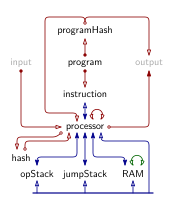
\includegraphics[keepaspectratio,width=0.7\textwidth]{src/img/aet-relations.pdf}
\end{center}
\ \\[2cm]
\begin{minipage}{0.5\textwidth}
    \rowcolors{2}{row2}{row1}
    \begin{tabular}{lrrr}
        \toprule
                  & base & ext & $\sum$ \\ \midrule
        Program   &    4 &   1 &      5 \\
        Processor &   42 &  11 &     53 \\
        OpStack   &    4 &   2 &      6 \\
        RAM       &    7 &   6 &     13 \\
        JumpStack &    5 &   2 &      7 \\
        Hash      &   66 &  19 &     85 \\
        Cascade   &    6 &   2 &      8 \\
        Lookup    &    4 &   2 &      6 \\
        U32       &   10 &   1 &     11 \\ \bottomrule
        $\sum$    &  148 &  46 &    194 \\
                  &      &     &
    \end{tabular}
\end{minipage}%
\begin{minipage}{0.5\textwidth}
    \hfill
    \rowcolors{2}{row2}{row1}
    \begin{tabular}{lrrrrr}
        \toprule
                    & init & cons & trans & term & $\sum$ \\ \midrule
        Program     &    2 &    1 &     3 &      &      6 \\
        Processor   &   37 &   11 &    73 &    1 &    122 \\
        OpStack     &    5 &      &     4 &      &      9 \\
        Ram         &    8 &      &    12 &    1 &     21 \\
        JumpStack   &    6 &      &     6 &      &     12 \\
        Hash        &   21 &   41 &    42 &      &    104 \\
        Cascade     &    2 &    1 &     3 &      &      6 \\
        Lookup      &    3 &    1 &     4 &    1 &      9 \\
        U32         &    1 &   14 &    21 &    2 &     38 \\
        Cross-Table &      &      &       &    1 &      1 \\ \bottomrule
        $\sum$      &   85 &   69 &   168 &    6 &    328
    \end{tabular}
\end{minipage}
\end{document}
